\graphicspath{{figures/analysis/}}
\chapter{Analysis}\label{ch:analysis}
To be able to both properly detect and track fish an evaluation of the state of the art solutions is necessary. This is done in regards to the already existing solution made by Loligo Systems called LoliTrack and other implementations of fish tracking in both two and three dimensions.

The chapter also presents setup and utility considerations.

\section{Fish Detection and Tracking}\label{sec:det_track}
As stated in \autoref{sec:loligo_res} Loligo Systems extracts BLOBs from a binary image to detect the fish in an aquarium. Using the binary image with noise reduction resembles a background subtraction, as the detector has a clear distinction between objects and empty space.

Background subtraction is a common detection technique for vision applications due to the separation between wanted objects and the rest of the scene in an image. A tracker which uses this is idTracker.

Another implementation of fish tracking is to separate each fish by determining the direction in which each fish is moving by determining where the head and tail of the fish is by splitting the body of the fish into rectangles.

\subsection{idTracker}
The tracker is able to track up to 20 objects in a scene from a video sequence by annotating specific fingerprints to each object and ID'ing it that way \citep{idtracker2014}.

\subsubsection{Detection}
Firstly each image from the video feed is normalised to its mean intensity, in which BLOBs with a mean pixel intensity outside of the set threshold are extracted. An optional background subtraction is possible using an average background image computed from the entire video.

The identification is done by comparing each BLOB extracted with reference images and compute the probability of a specific BLOB belonging to the correct ID.

\subsubsection{Tracking}
The tracking is done while detecting as any frame without any type of occlusion or collision are stored and used for tracking while the occlusions are handled. The saved frames are also used as references during occlusion handling. The trajectories are created using the coordinates extracted from the detection.

\subsection{Rectangle Body Modelling}
According to \cite{HongWang2016} the fish body is split into 8 rectangles with the same length but decreasing width to match the curvature of the fish body going from head to tail. \autoref{fig:rect-flow} shows a flow diagram of the detection and tracking process. The solution relies on the head region of fish is somewhat rigid when using a top-view.

\begin{figure}[H]
	\centering
	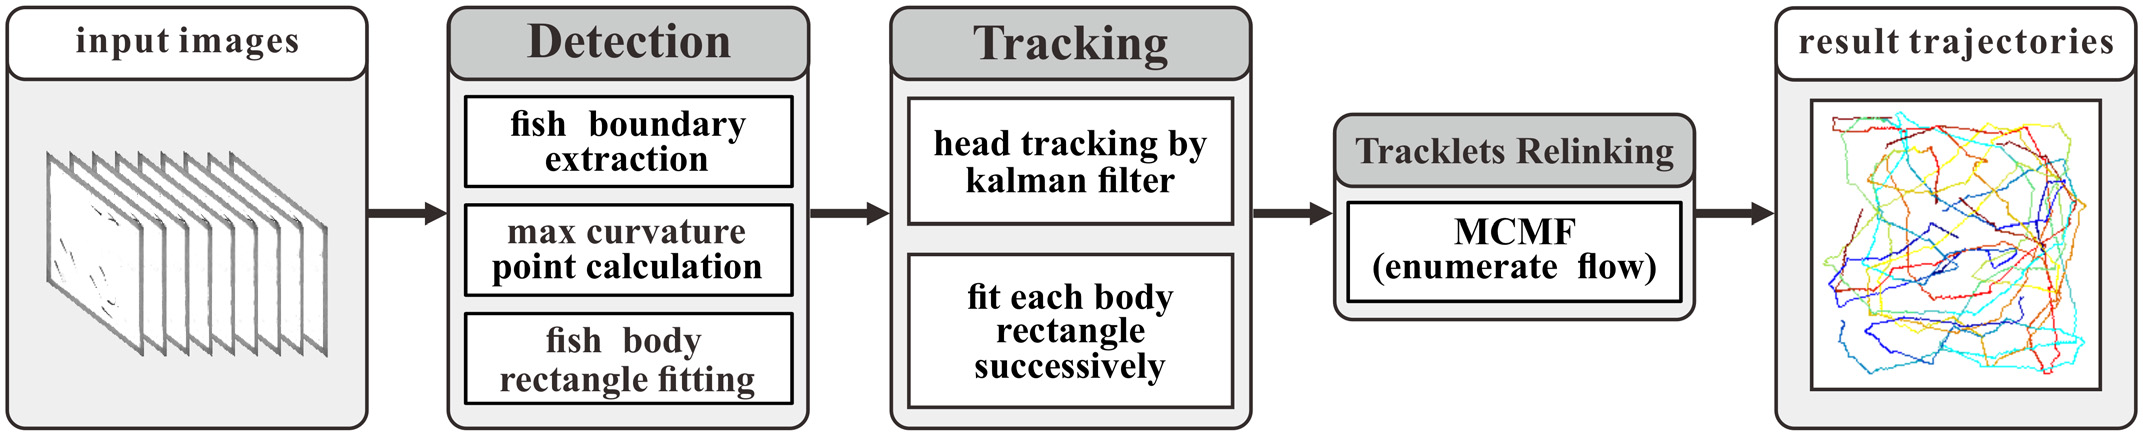
\includegraphics[width=\textwidth]{rect-flow}
	\caption{Flow diagram of the rectangle body modelling fish tracking \citep{HongWang2016}}
	\label{fig:rect-flow}
\end{figure}

\subsubsection{Detection}
The implementation firstly makes a background subtraction with a background image made in the same way as from idTracker. And then converted to a binary image by using a threshold. From there the boundary of each fish is extracted.

The curvature of the fish body is computed along with detection of the nose point of the fish. by locating the two local maximums on the fish; one on the nose of the fish, which is the lower one, and one on the tail.

Head orientation is found using two points on the head curvature. The orientation is then defined as a direction perpendicular to the line between the two points. With the nose point and head orientation it is possible to place the first rectangle.

Pose estimation of the fish is done based on rectangle chain fitting. Each rectangle is fixed to a joint on the previous rectangle. The following rectangle is then rotated around the joint in a fixed amount of random angles between $0$ and $2\pi$. The rectangles are of fixed sizes and the rectangle which covers the fish the best is chosen. An example of the rectangles covering the fish is shown in \autoref{fig:rect-fish}.

\begin{figure}[h]
  \centering
  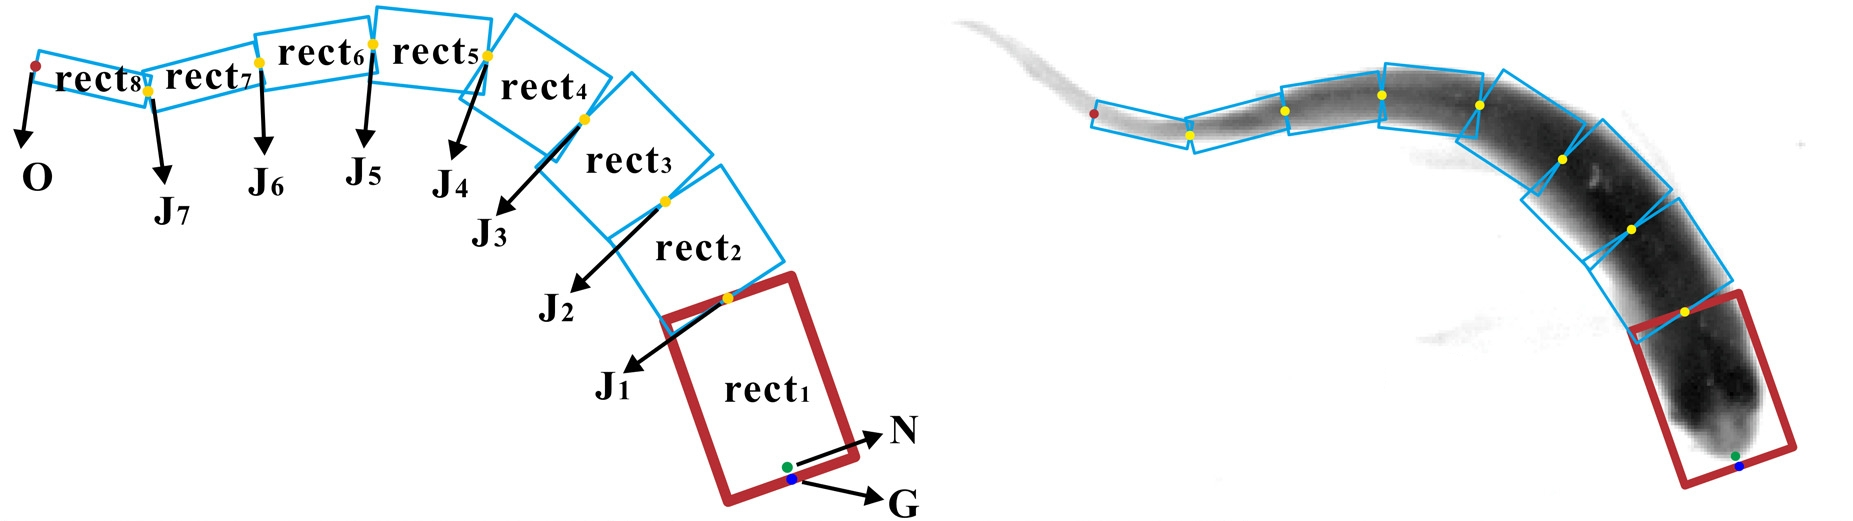
\includegraphics[width=\textwidth]{rect-fish}
  \caption{Example of rectangles covering the fish to define shape \citep{HongWang2016}}
  \label{fig:rect-fish}
\end{figure}

\subsubsection{Tracking}
As previously mentioned, the solution is based on the head region of the fish being somewhat rigid. When tracking, \cite{HongWang2016} firstly tracks the head of the fish using a Kalman filter. 

Data association is securing one tracker is associated with only one measurement. \cite{HongWang2016} formulates this as a global optimisation problem and employs the Hungarian algorithm to solve the problem.

When the head location and orientation is found the rectangle chain fitting is done as described previously. If the eight rectangles cover less than $80\%$ in a frame, the tracker is terminated, which can lead to trajectories being split, needing tracklets re-linking.

The re-linking is classified as a minimum cost maximum flow problem to solve re-linking to handle potential occlusions.

\subsection{Head Region Detection}
\cite{Qian2014} propose a solution which is targeted at tracking multiple fish swimming in shallow water while handling frequent occlusions. By using the rigidity of the head of the fish the solution uses the shape of the head in a combination with feature extraction of each fish to detect and track each fish individually. An overview flow diagram of the implementation, from the article, is shown in \autoref{fig:head_det}.

\begin{figure}[H]
	\centering
	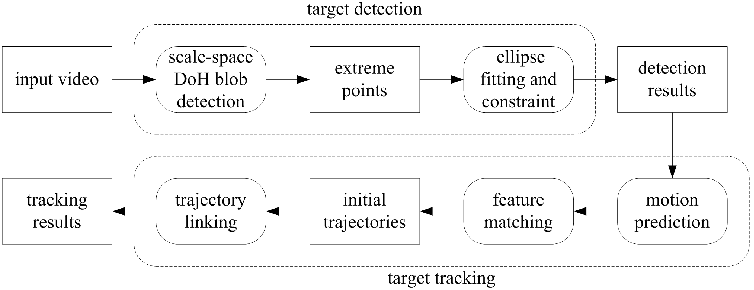
\includegraphics[width=\textwidth]{head-det_ov}
	\caption{Overview flow diagram of the implementation \citep{Qian2014}}
	\label{fig:head_det}
\end{figure}

\subsubsection{Detection}
The detection implemented is using both a geometric feature and a local feature. The detection consists of two parts; a scale-space \gls{doh} blob detection, and ellipse fitting and constraint.

By using a high contrast image, the pixels of the fish is darker than the background in the image. This is used together with the partial elliptical shape of the fish head and the decreasing width of the fish from head to tail. The blob of the fish is extracted using \gls{doh}, as this is a strong scale-space blob detection able to suppress slim blobs in the image \citep{Qian2014}.

Ellipse fitting is done to be able to locate the head of a fish properly, as an extreme point found using \gls{doh} blob detection may appear other places than the one on the fish head. The fitting is done according to the grey-scale change of each extreme point region. To avoid noise a width threshold is set to th ellipse used. Even still, extra points can occur and to combat these contrast constraining is done. This is done by firstly image segmentation by thresholding to a binary image. The best thresholding value is then used as a parameter used to determine if a head is located or not, based on the contrast difference between the head and other body parts of the fish, as the head is proven darker than the rest of the fish \citep{Qian2014}.

Should a duplicate detection occur, meaning having two detections in one head region, an angle constraint is used. If the angle between the two detections is higher than $30 \degree$ the detection with the higher contrast is kept as the head.

\subsubsection{Tracking}
When detection is finished, each target is tracked. \cite{Qian2014} splits the tracking in three parts: motion prediction, feature matching, and trajectory linking.

The motion prediction is done using a Kalman filter to predict the motion state from the state vector: $ x_k = (x,y,v_x,v_y) $, where $x$ and $y$ are the head point coordinates and $v_x$ and $ v_y $ are the speeds in the speeds in their respective directions. As the fish can move very sporadic, a constant velocity model can lead to errors. To account for this plausible error \cite{Qian2014} implements a compensation window prescribing the detected ellipse's direction inside a quarter circle.

The feature matching is based on the head region of the fish using width, area, and greyscale information, which limits the solution to a low water setup, as the vertical swimming possibilities are very limited for the fish, limiting the size variations of the fish. The width is found by contouring the fish and drawing a line perpendicular to the direction vector from the ellipse centre and measuring the length of that line. The area used, is the entire matching region used. Greyscale matching is based on a histogram of the matching region. An example of the motion prediction compensation window and feature matching region is shown in \autoref{fig:head_det_track}.

\begin{figure}[H]
	\centering
	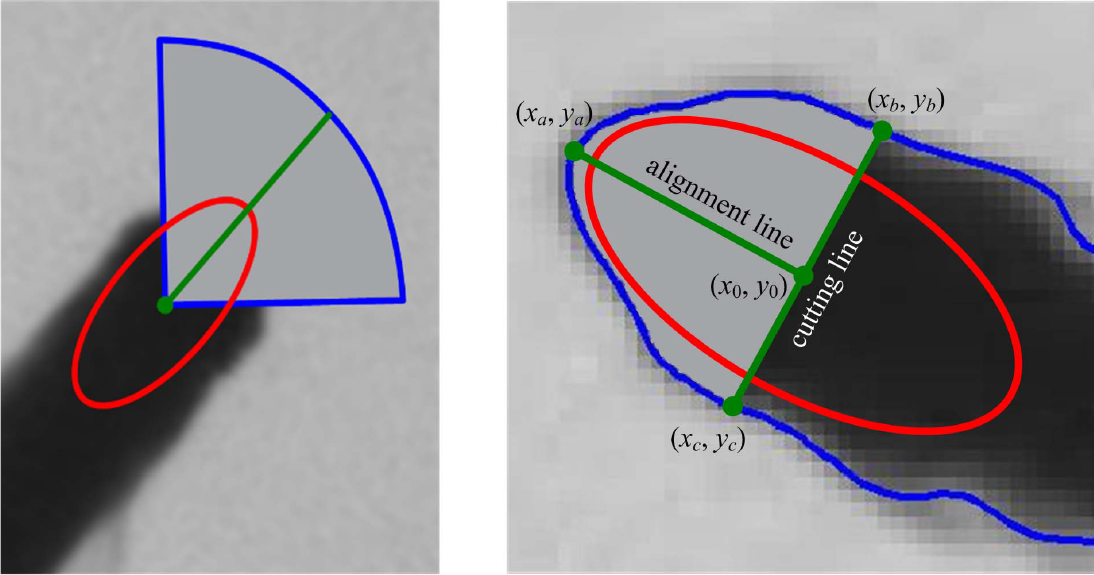
\includegraphics[width=0.7\textwidth]{head_det_track}
	\caption{Example of the motion prediction compensation window and feature matching region \citep{Qian2014}}
	\label{fig:head_det_track}
\end{figure}

Trajectory linking is done to check if two trajectory fragments belong together. If the two fragments meets both the time constraint and the space constraint made, feature matching is done on both fragments to further determine if the two fragments should be linked, as belonging to one fish.

\section{Data Acquirement}
In order to do tracking of the fish, data needs to be sampled. This is done in cooperation with Loligo Systems at their offices in Viborg, Denmark.

\subsection{Recording Set-up}
The cameras used are two identical iDS UI-3370CP Rev. 2 cameras, able to record at $80$ frames per second at full resolution of $ 2048\times2048 $ pixels. The camera is fitted with a Kowa LM25HC lens to be able to adjust optical zoom and focus. The higher the resolution of the camera, the lower amount of frames it is able to record. Recording in full high definition of $1920 \times 1080$ yields $50$ frames per second, which enables the camera to capture a lot of the fish's sporadic movements.

When recording to achieve a stereo vision, the cameras are placed at the same distance from the centre point of the aquarium to opposite sides. Both cameras are placed above the aquarium at the same height. An overview example of the set-up is shown in \autoref{fig:cam_setup}. The figure also includes the set up when using only one camera. In this instance, the camera is centred over the aquarium and placed at a height in which all the water in the camera is captured. 

\begin{figure}
	\centering
	\begin{subfigure}{0.4\textwidth}
		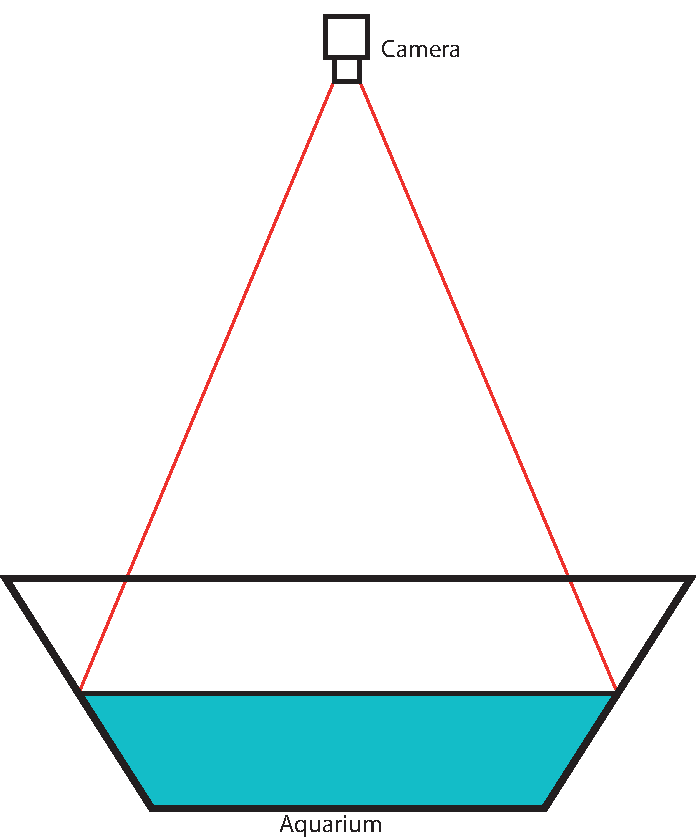
\includegraphics[width=\textwidth]{single_setup}
		\caption{Set up of video capture using a single camera centred above the aquarium}
		\label{fig:single_setup}
	\end{subfigure}
	\begin{subfigure}{0.4\textwidth}
		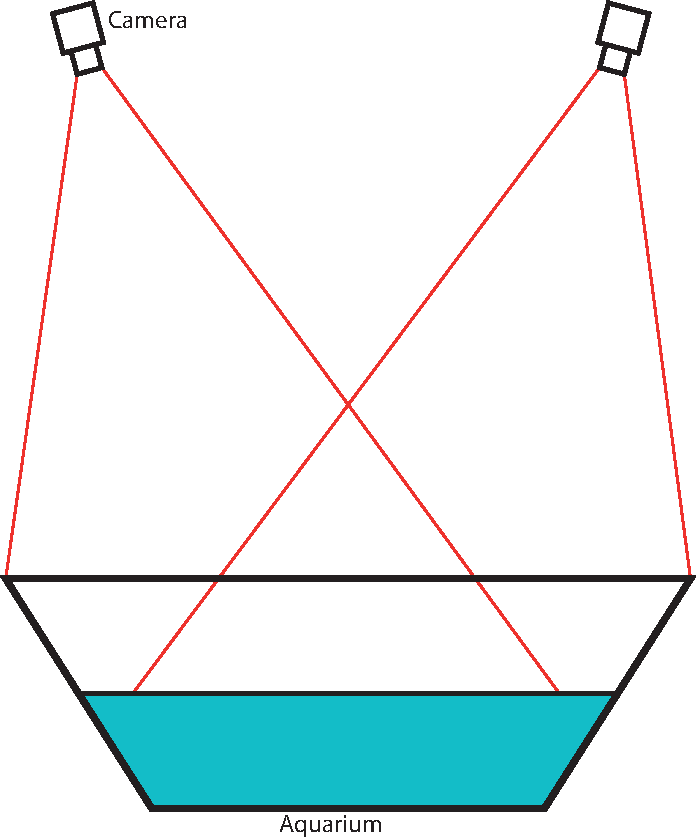
\includegraphics[width=\textwidth]{duo_setup}
		\caption{Set up of stereo video capture using two cameras offset equally from the centre of the aquarium}
		\label{fig:duo_setup}
	\end{subfigure}
\caption{The two set ups used to capture video data of the fish}
\label{fig:cam_setup}
\end{figure}

\section{Delimitations}
Due to time constraints, it was chosen to focus on 2D-tracking instead of 3D-tracking. Furthermore, to be able to implement a 3D-tracking system to match Loligo System's aim, the system had to be robust to multiple different types of shapes. Due to this, a robust 2D-tracking implementation was needed before any 3D-tracking could be implemented, as a 3D solution in theory is a 2D-tracking used with two cameras and combining the acquired data from the two cameras.

As presented in \autoref{sec:det_track} there exist multiple detection and tracking algorithms for 2D. Due to the multiple tracking solutions existing, it is chosen to focus on a solution able to detect whether an occlusion is occurring.\\

With this a problem statement is made in the following chapter.